\documentclass[a4paper,twoside]{article}
\usepackage[T1]{fontenc}
\usepackage{graphicx}
\usepackage{graphics}
\usepackage{float}
\usepackage[cm]{fullpage}
\pagestyle{myheadings}
\usepackage{etoolbox}
\usepackage{setspace} 
\usepackage{lipsum} 
\usepackage[bahasa]{babel}
\setlength{\headsep}{30pt}
\usepackage[inner=2cm,outer=2.5cm,top=2.5cm,bottom=2cm]{geometry} %margin
% \pagestyle{empty}

\makeatletter
\renewcommand{\@maketitle} {\begin{center} {\LARGE \textbf{ \textsc{\@title}} \par} \bigskip {\large \textbf{\textsc{\@author}} }\end{center} }
\renewcommand{\thispagestyle}[1]{}
<<<<<<< HEAD
\markright{\textbf{\textsc{AIF401/AIF402 \textemdash Rencana Kerja Skripsi \textemdash Sem. Ganjil 2018/2019}}}
=======
\markright{\textbf{\textsc{AIF401/AIF402 \textemdash Rencana Kerja Skripsi \textemdash Sem. Genap 2016/2017}}}
>>>>>>> ea0203ebe687b74b9baf98a93d09fd0166560bd2

\newcommand{\HRule}{\rule{\linewidth}{0.4mm}}
\renewcommand{\baselinestretch}{1}
\setlength{\parindent}{0 pt}
\setlength{\parskip}{6 pt}

\onehalfspacing
 
\begin{document}

\title{\@judultopik}
\author{\nama \textendash \@npm} 

%tulis nama dan NPM anda di sini:
\newcommand{\nama}{Evelyn Wijaya}
\newcommand{\@npm}{2015730030}
\newcommand{\@judultopik}{Open Source Snake 360} % Judul/topik anda
\newcommand{\jumpemb}{1} % Jumlah pembimbing, 1 atau 2
<<<<<<< HEAD
\newcommand{\tanggal}{07/09/2018}
=======
\newcommand{\tanggal}{01/01/1900}
>>>>>>> ea0203ebe687b74b9baf98a93d09fd0166560bd2

% Dokumen hasil template ini harus dicetak bolak-balik !!!!

\maketitle

\pagenumbering{arabic}

\section{Deskripsi}
\textit{Snake} merupakan sebuah permainan yang pertama kali dibuat oleh Peter Trefonas pada tahun 1978. Konsep \textit{Snake} pertama kali berasal dari permainan arkade yaitu \textit{Blockade}. Pada saat itu, \textit{Snake} hanya dapat dimainkan pada komputer pribadi saja. Pada tahun 1997, \textit{Snake} dapat dimainkan pada telepon genggam \textit{Nokia}\footnote{https://en.wikipedia.org/wiki/Snake\_(video\_ game\_ genre)}. Cara bermainya cukup mudah yaitu pemain mengendalikan ular untuk mendapatkan makanan tanpa menabrak rintangan atau ular itu sendiri. Setiap memakan makanan, pemain akan mendapat skor dan tubuh ular akan memanjang. Apabila ular tersebut menabrak dirinya sendiri atau menabrak rintangan, maka permainan selesai.\\\\
HTML5 adalah sebuah bahasa markah yang digunakan untuk membuat sebuah halaman \textit{web}. HTML5 merupakan versi kelima dan terbaru. HTML5 memiliki beberapa API (\textit{Application Programming Interface}) baru, salah satunya adalah \textit{canvas}\footnote{https://en.wikipedia.org/wiki/HTML5}. \textit{Canvas} adalah sebuah wadah untuk menggambar bentuk 2D dan menambah sebuah gambar pada halaman \textit{web}. Dibutuhkan \textit{JavaScript} untuk menggambar pada \textit{canvas}\footnote{https://www.w3schools.com/html/html5\_canvas.asp}.\\\\
Sekarang, sudah banyak sekali permainan \textit{Snake} yang dapat dimainkan di \textit{smartphone} dan \textit{web}. Bahkan pergerakan ular juga tidak hanya 4 arah saja (atas, bawah, kiri dan kanan), tetapi sudah dapat bergerak ke segala arah. Selain itu, ada permainan \textit{Snake} yang dapat dimainkan lebih dari 1 orang, contohnya adalah Slither.io. Pada skripsi ini akan dibuat permainan \textit{Snake} yang ularnya dapat bergerak ke segala arah dan orang lain dapat menambahkan pilihan labirin. Permainan \textit{Snake} akan dibuat menggunakan HTML5 serta orang lain dapat menambah pilihan labirin menggunakan mekanisme \textit{pull request} pada \textit{Github}.

\begin{figure}[H]
	\centering
	\begin{minipage}{.5\textwidth}
		\caption{Pergerakan ular ke segala arah}
		\centering
		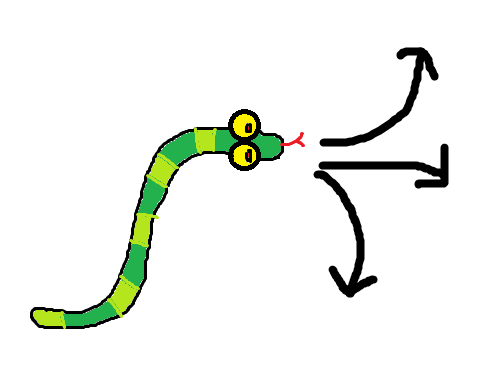
\includegraphics[width=0.5\textwidth]{snake.png}
	\end{minipage}%
	\begin{minipage}{.5\textwidth}
		\caption{Permainan \textit{Snake} pada telepon genggam \textit{Nokia}}
		\centering
		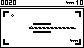
\includegraphics[width=0.6\textwidth]{nokiaSnake.png}
	\end{minipage}
\end{figure}

\section{Rumusan Masalah}
\begin{itemize}
	\item Bagaimana membangun permainan \textit{Snake} menggunakan HTML5? 
	\item Bagaimana cara menyimpan labirin pada file eksternal?
	\item Bagaimana cara menggunakan \textit{pull request} pada \textit{Github} agar orang lain dapat menambahkan labirin?
\end{itemize}

\section{Tujuan}
\begin{itemize}
	\item Dapat membangun permainan \textit{Snake} menggunakan HTML5. 
	\item Dapat menyimpan labirin pada file eksternal.
	\item Dapat menggunakan \textit{pull request} pada \textit{Github} agar orang lain dapat menambahkan labirin.
\end{itemize}

\section{Deskripsi Perangkat Lunak}
Perangkat lunak akhir yang akan dibuat memiliki fitur minimal sebagai berikut:
\begin{itemize}
	\item Pengguna dapat menggerakan ular ke segala arah dalam permainan \textit{Snake} tersebut. 
	\item Pengguna dapat menambahkan labirin menggunakan mekanisme \textit{pull request} pada \textit{Github} yang dapat disimpan pada file eksternal.
\end{itemize}

\section{Detail Pengerjaan Skripsi}
Bagian-bagian pekerjaan skripsi ini adalah sebagai berikut :
	\begin{enumerate}
		\item Melakukan studi literatur mengenai HTML5, \textit{Javascript, jQuery} dan \textit{pull request} pada \textit{Github}.
		\item Melakukan analisis dan menentukan objek-objek pada permainan \textit{Snake}.
		\item Merancang alogritma untuk menggambar tubuh ular, pergerakan ular dan membuat labirin.
		\item Mengimplentasikan keseluruhan algoritma.
		\item Menambahkan labirin menggunakan \textit{pull request} pada \textit{Github}.
		\item Melakukan pengujian dan \textit{debugging}.
		\item Menulis dokumen skripsi.
	\end{enumerate}

\section{Rencana Kerja}
Rincian capaian yang direncanakan di Skripsi 1 adalah sebagai berikut:
\begin{enumerate}
<<<<<<< HEAD
\item Melakukan studi literatur mengenai HTML5, \textit{Javascript, jQuery} dan \textit{pull request Github}.
\item Melakukan analisis dan menentukan objek-objek pada permainan \textit{Snake}.
\item Merancang algoritma untuk menggambar tubuh ular dan pergerakan ular.
\item Mengimplementasikan algoritma untuk menggambar tubuh ular dan pergerakan ular.
\item Menulis bab 1 dan bab 2.
=======
\item
\item
\item
>>>>>>> ea0203ebe687b74b9baf98a93d09fd0166560bd2
\end{enumerate}

Sedangkan yang akan diselesaikan di Skripsi 2 adalah sebagai berikut:
\begin{enumerate}
<<<<<<< HEAD
\item Merancang algoritma untuk membuat labirin. 
\item Mengimplementasikan algoritma untuk membuat labirin.
\item Menambahkan labirin menggunakan \textit{pull request} pada \textit{Github}.
\item Melakukan pengujian dan debugging.
\item Melanjutkan dokumen skripsi.
=======
\item
\item
\item
>>>>>>> ea0203ebe687b74b9baf98a93d09fd0166560bd2
\end{enumerate}

\vspace{1cm}
\centering Bandung, \tanggal\\
\vspace{2cm} \nama \\ 
\vspace{1cm}

Menyetujui, \\
\ifdefstring{\jumpemb}{2}{
\vspace{1.5cm}
\begin{centering} Menyetujui,\\ \end{centering} \vspace{0.75cm}
\begin{minipage}[b]{0.45\linewidth}
% \centering Bandung, \makebox[0.5cm]{\hrulefill}/\makebox[0.5cm]{\hrulefill}/2013 \\
\vspace{2cm} Nama: \makebox[3cm]{\hrulefill}\\ Pembimbing Utama
\end{minipage} \hspace{0.5cm}
\begin{minipage}[b]{0.45\linewidth}
% \centering Bandung, \makebox[0.5cm]{\hrulefill}/\makebox[0.5cm]{\hrulefill}/2013\\
\vspace{2cm} Nama: \makebox[3cm]{\hrulefill}\\ Pembimbing Pendamping
\end{minipage}
\vspace{0.5cm}
}{
% \centering Bandung, \makebox[0.5cm]{\hrulefill}/\makebox[0.5cm]{\hrulefill}/2013\\
\vspace{2cm} Nama: \makebox[3cm]{\hrulefill}\\ Pembimbing Tunggal
}
\end{document}

